\section{Listen}
\label{lists-main}
Listen sind etablierte \gls{ui} Komponenten, die dem Anwender eine Vielzahl gleichartiger Elemente präsentieren. Die Elemente können unterschiedlich angeordnet sein und vom Anwender mittels Gesten durchlaufen werden (Scrollen). Der Aufbau und die Struktur von Listen unterscheiden sich zum Teil stark voneinander. Man kann Listen in Bezug auf die Anordnung der Elemente (Horizontal, Vertikal, Raster) oder dem Verhalten beim Befüllen und Scrollen unterscheiden. Eine häufig verwendete und auch von Ionic unterstütze Variante ist die horizontale Anordnung der Elemente. Die im Folgenden betrachteten Listen und Tests fokussieren sich dabei auf diese Art von Listen.
\begin{table}[h]
	\centering
	\begin{tabular}{llp{8cm}}
		\textbf{Nr.} & \textbf{Kriterium} & \textbf{Beschreibung}\\
		\hline
		1 & Seitenwechsel & Die Performance beim Wechseln auf eine Seite wird durch die Größe einer Liste beeinflusst. Wechselt der Nutzer auf eine Seite mit vielen Listenelemente, dauert dieser Seitenübergang entsprechend länger als bei wenigen Listenelementen.\\
		2 & Scrollen & Für das Nutzererlebnis ist es wichtig, dass der Anwender eine Liste ohne Verzögerungen durchlaufen kann.\\
		3 & Arbeitsspeicher & Enthält eine Liste viele Elemente, wird auch entsprechend viel Arbeitsspeicher benötigt. Wie in Abschnitt \ref{performance-categories-web} beschrieben, kann ein ausgelasteter Arbeitsspeicher den Druck auf die Performance durch den Garbage Collector erhöhen.\\
		4 & Two-Way-Databinding & Zur automatischen Synchronisation von Views und Models muss eine Liste bei jedem \emph{\$digest}-Zyklus auf Änderungen geprüft werden. Die Listenimplementierung und die Anzahl der Elemente in der Liste beeinflussen maßgeblich die Performance dieses Prüfvorgangs.\\
	\end{tabular}
	\caption{Seitenübergänge, Listen Kriterien}
	\label{su-lists-criterias}	
\end{table}
\\\\
Listen dienen der Anzeige von gleichartigen Elementen. Die Anzahl der Elemente ist dabei ausschlaggebend für die Performance der Liste. Denn Listenelemente werden durch \gls{dom}-Elemente repräsentiert und ihre Anzahl beeinflusst, wie in Abschnitt \ref{browser-engines} beschrieben, maßgeblich die Performance beim Layouten und Rendern der Seite. Wenn sich zu viele Elemente in einer Liste befinden, kann es schnell zu Problemen in der Performance kommen. Der Begriff \glqq Viele\grqq{} ist dabei Variabel und hängt unter anderem von der Leistungsfähigkeit des jeweiligen Gerätes ab. Bei Apps ist dieser Wert dadurch um einiges geringer als bei herkömmlichen Webseiten. Aus diesem Grund ist es wichtig eine Liste möglichst ressourcensparend und für den jeweiligen Einsatz optimal zu implementieren. In den folgenden Abschnitten werden daher zunächst verschiedene Listenimplementierungen analysiert und anschließend durch Tests hinsichtlich der Performance anhand von vier Kriterien untersucht (Tabelle \ref{su-lists-criterias}). Jedes dieser Kriterien steht im Zusammenhang mit der Performance oder dem Nutzererlebnis bei der Verwendung der Liste. 

\subsection{Arten}
In diesem Abschnitt werden vier von AngularJS und Ionic zur Verfügung gestellte Listenimplementierungen analysiert. Die ersten beiden Varianten \glqq statische Listen\grqq{} und \glqq dynamische Listen\grqq{} bezeichnen grundsätzliche Verfahren für Listen in AngularJS. Die anderen beiden Varianten, \gls{is} und \gls{vs}, umfassen erweiterte Konzepte für Listen und werden von Ionic zur Verfügung gestellt.

\subsubsection{Dynamische Listen}
In AngularJS können Listen über die Direktive \emph{ngRepeat} implementieren werden. Diese Direktive kopiert das \gls{dom}-Element, auf das es angewendet wird, für jedes Element eines JavaScript Arrays (Listing \ref{lists-dynamic}). Durch das AngularJS Two-Way-Databinding wird diese visuelle Liste mit dem JavaScript Array synchronisiert. Neue Elemente im Array werden demnach automatisch in den \gls{dom} eingefügt. Diese Art von Liste wird als dynamische Liste bezeichnet. Veränderungen an den Daten im Model wirken sich demnach auf die Anzeige aus. Der Vorteil dieser Art von Liste liegt in der simplen Implementierung. Der Nachteil ist die schlechtere Performance durch die automatische Synchronisation für das Two-Way-Databinding. Je mehr Elemente sich in dieser Liste befinden, desto länger dauert der \emph{\$digest}-Zyklus.\\\\
\begin{lstlisting}[language=HTML,style=ionicHtmlStyle,caption={Dynamische Listen mit AngularJS}\label{lists-dynamic}]
<ion-list>
	<ion-item ng-repeat="item in items">
		<book book="item"></book>
	</ion-item>
</ion-list>
\end{lstlisting}

\subsubsection{Statische Listen}
Im Gegensatz zu einer dynamischen Liste ist die Eigenschaft einer statischen Liste, dass sich die Anzahl und Reihenfolge von Elementen zur Laufzeit nicht ändert. Bei solch einer Liste kann, wie in Abschnitt \ref{dv-main} beschrieben, Zeit eingespart werden, indem Prüfvorgänge für das Two-Way-Databinding entfallen. AngularJS prüft dadurch zur Laufzeit nicht, ob sich der Inhalt des JavaScript-Arrays geändert hat. Der Vorteil ist die einfache Implementierung und die bessere Performance bei vielen Elementen im Vergleich zur dynamischen Liste. Für die statische Liste wird das AngularJS One-Time Binding verwendet. Dies wurde bereits in Abschnitt \ref{dyn-views-onetimebinding} näher beschrieben (Listing \ref{lists-static}).\cite{AJSOneTimeBinding}
\begin{lstlisting}[language=HTML,style=ionicHtmlStyle,caption={Statische Listen mit AngularJS}\label{lists-static}]
<ion-list>
	<ion-item ng-repeat="item in ::items">
		<book book="item"></book>
	</ion-item>
</ion-list>
\end{lstlisting}

\subsubsection{Infinite Scrolling}
\gls{is} (\glqq unendliches scrollen\grqq) benennt ein Verfahren, bei dem eine Liste zur Laufzeit beim Scrollen durch den Anwender um weitere Elemente ergänzt wird. Zu Beginn befindet sich nur eine begrenzte Anzahl von Elementen in der Liste. Scrollt der Anwender an das Ende, werden automatisch weitere Elemente angehängt. Dieser Vorgang wird so lange wiederholt, bis das tatsächliche Ende der Liste erreicht ist. Für den Anwender erscheint die Liste als von Anfang an vollständig. Der Vorteil dieses Verfahrens ist die Tatsache, dass sich zu Beginn nur eine begrenzte Anzahl von Elementen in der Liste befinden. Dies ist optimal für den Seitenwechsel, den Arbeitsspeicherverbrauch und das Two-Way-Databinding. Erst nach dem Scrollen an das Ende der Liste verhält sich dieses Verfahren wie eine einfache dynamische Liste. Ein Nachteil ist das Hinzufügen neuer Elemente beim Scrollen, wodurch das Nutzererlebnis durch Verzögerungen beeinträchtigt werden kann.\\\\
\begin{lstlisting}[language=HTML,style=ionicHtmlStyle,caption={Infinite Scrolling mit Ionic (View)}\label{lists-infinite}]
<ion-list>
	<ion-item ng-repeat="item in items">
		<book book="item" />
	</ion-item>
</ion-list>
<ion-infinite-scroll on-infinite="loadMore()" distance="1%" />
\end{lstlisting}
Mittels der Direktive \emph{ionInfiniteScroll} lässt sich dieses Verfahren mit Ionic implementieren. In Kombination mit der Direktive \emph{ngRepeat} kann eine Liste mit \gls{is} Eigenschaften realisiert werden. Überschreitet der Anwender beim Scrollen eine Distanz zum Ende der Seite, ruft Ionic eine vom Entwickler bereitgestellte Funktion auf. In dieser Funktion können zusätzliche Elemente an die Liste angehängt werden. 
\begin{lstlisting}[language=JavaScript, caption={Infinite Scrolling mit Ionic (Controller)}\label{su-rr}]
$scope.items = []; $scope.maxItems = ...;
$scope.loadMore = function () {
	for(var i = 0; i < ...; i++)
		$scope.items.push(...);
	$scope.$broadcast('scroll.infiniteScrollComplete');
};
\end{lstlisting}

\subsubsection{Virtual Scrolling}
\gls{vs} bezeichnet ein Verfahren, bei dem sich zu jedem Zeitpunkt nur eine feste Anzahl von Elementen in einer visuellen Liste befinden. Das Ziel ist es, möglichst wenig \gls{dom}-Elemente gleichzeitig im \gls{dom} zu verwalten. Dabei werden nur diejenigen Elemente der Liste in den DOM eingefügt, die sich im für den Anwender sichtbaren Bereich befinden (Viewport). Scrollt der Anwender durch die Liste, werden Elemente oberhalb des Viewport aus dem \gls{dom} entfernt und unterhalb eingefügt. Um Verzögerungen beim Scrollen zu vermeiden, befinden sich oberhalb und unterhalb des Viewport jeweils ein kleiner Bereich mit Elementen als Puffer. Um die Speicherauslastung zu verringern, werden \gls{dom}-Elemente nach der Verwendung zwischengespeichert und bei Bedarf wiederverwendet. Damit die Position einzelner Elemente korrekt berechnet werden kann, ist die konkrete Größe jedes Elementes erforderlich. Bei gleich großen Elementen ermittelt AngularJS die Größe automatisch anhand des ersten Elementes. 
\begin{figure}[h]
	\centering
	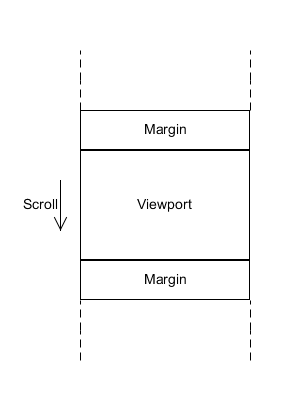
\includegraphics[scale=0.4]{Bilder/VirtualScrolling.png}
	\caption{Konzept Virtual Scrolling}
	\label{konzept-virtualscrolling}
\end{figure}
Der klare Vorteil von \gls{vs} ist die permanent kleine Anzahl von Elementen, die sich zeitgleich im \gls{dom} befindet. Dies beeinflusst die Ladezeit beim Seitenwechsel, die Arbeitsspeicherauslastung und den \emph{\$digest}-Zyklus positiv. Ein Nachteil dieses Verfahrens ist die Tatsache, dass die Größe jedes Elementes der Liste bekannt sein muss. Bei unterschiedlich großen Elementen kann dies zu einer verschlechterten Performance durch die Berechnung führen. Außerdem gilt es als schlechter Stil, die Größe von \gls{ui}-Komponenten fest in einer Anwendung zu hinterlegen.

\subsection{Analyse}
Im Rahmen dieser Analyse sollen die betrachteten Listenarten hinsichtlich der in Abschnitt \ref{lists-main} genannten Kriterien untersucht werden. Das Ziel ist es, für jeden Anwendungsfall die optimale Listenart zu ermitteln. Für den Test werden zwei weitere Kriterien definiert. Zum einen sollen die Listen mit einer unterschiedlichen Anzahl von Elementen und zum anderen mit unterschiedlich komplexen Elementen getestet werden. Denn komplexe \glspl{Template} erzeugen mehr \gls{dom}-Elemente als simple \glspl{Template}. Dies kann die Performance und die optimale Listenart beeinflussen. Für die Anzahl der Elemente wird eine Abstufung von 10, 50, 100 festgelegt. Hinsichtlich der Komplexität werden 2 DOM-Elemente für die simple Variante und 10 DOM-Elemente für die komplexe Variante definiert. Durch diese Kriterien ergeben sich 24 Messungen pro Android Version und Listenart. Die Arbeitsspeicherauslastung kann nicht auf den mobilen Geräten untersucht werden. Die APIs werden zwar durch Chromium und Webkit bereitgestellt, aufgrund von Sicherheitsaspekten liefern sie jedoch nur beim manuellen Starten des Browsers mit entsprechenden Kommandozeilenargumenten korrekte Ergebnisse. Dieses Kriterium wird daher nicht weiter betrachtet. 
\\\\
Für die verschiedenen Listenarten, sowie die unterschiedlichen Kriterien wurden entsprechende Module in der Testanwendung angelegt. Für jede Listenart entstehen dabei zwei Module. Im ersten Modul wird gemessen, wie viel Zeit ein Wechsel auf die Seite mit der jeweiligen Liste benötigt. Im zweiten Modul wird das Scrollen simuliert und die Zeit für einen \emph{\$digest}-Zyklus gemessen. Abbildung \ref{lists-test-prozess} zeigt die Abläufe der einzelnen Tests. Für die Simulation des Scrollens wird auf BenchmarkJS verzichtet. An dieser Stelle soll der Anwender simuliert werden und Verzögerungen beim Scrollen mit in die Zeitmessung einfließen. Beim Beginn und Ende der Simulation wird daher die Zeit gestoppt und die Differenz als Messungen herangezogen.  
\begin{figure}[h]
	\centering
	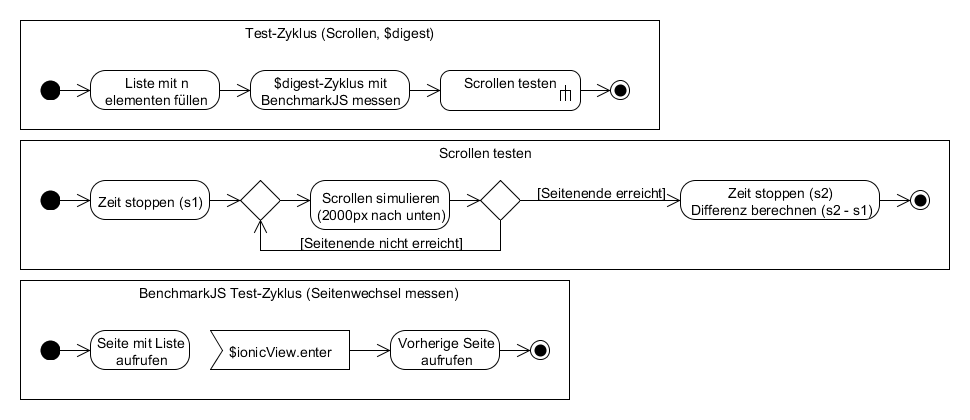
\includegraphics[scale=0.4]{Bilder/UML-Activity-Listen.png}
	\caption{Testablauf für Listen anhand vorher definierter Kriterien}
	\label{lists-test-prozess}
\end{figure}

\subsubsection{Kriterium - Seitenwechsel}
Das erste Kriterium zielt auf die Verbesserung der Performance bei Seitenwechseln. Je schneller eine Seite geladen wird, desto positiver ist das Nutzererlebnis. Es gilt demnach zu untersuchen, welche Listenart hinsichtlich der Seitenwechsel die beste Performance liefert. Abbildung \ref{lists-runtime-pagetransitions} zeigt das Ergebnis dieser Analyse. Aus diesem Diagramm wird ersichtlich, dass der Seitenwechsel bei statischen und dynamischen Listen ab einer bestimmten Listengröße wesentlich langsamer ist als bei Listen auf Basis der \gls{is} und \gls{vs} Technik. Außerdem wird deutlich, dass mit zunehmender Listengröße die Performance weiter abnimmt. Bei den letzten beiden Techniken bleibt die Geschwindigkeit aufgrund ihrer Eigenschaften relativ konstant. Die Schwelle, ab der \gls{is} und \gls{vs} Performancetechnisch überlegen sind, liegt in etwa bei 10 Listen-Elementen. Eine Abweichung kann aufgrund der Komplexität der Elemente möglich sein. Bei \gls{is} hängt dieser Wert zusätzlich von der konfigurierten Mengen an Elementen ab, die sich zu Beginn in der Liste befinden. In diesen Tests wurde dafür der Wert 10 verwendet. 
\\\\
Es lässt sich demzufolge festhalten, dass der Einsatz von \gls{is} und \gls{vs} bereits bei 10 Elementen die Performance für Seitenwechseln positiv beeinflusst. Das Optimierungspotential ist enorm. Die größte Steigerung liegt in den Messungen bei 518\% zwischen einer statischen Liste und der \gls{vs} Technik bei Android 4.4.4. Im Vergleich zwischen den beiden Android Versionen zeigt sich, dass die ältere Version 4.3 in allen Messungen eine bessere Performance aufweist.   
\begin{figure}[h]
	\centering
	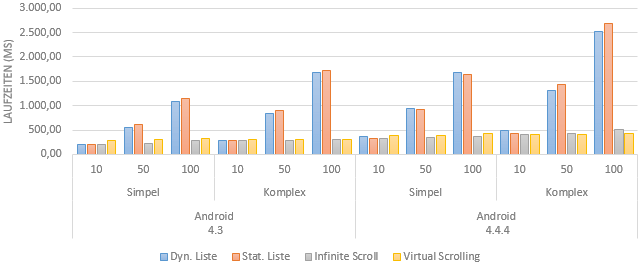
\includegraphics[scale=0.7]{Bilder/Diagramme/List-PageTransition.png}
	\caption{Listen - Laufzeitmessung Seitenübergänge}
	\label{lists-runtime-pagetransitions}
\end{figure}

\subsubsection{Kriterium - Scrollen}
Das zweite untersuchte Kriterium befasst sich mit der Geschwindigkeit beim Scrollen durch eine Liste. Jede Listenart wurde dazu mit unterschiedlich vielen Elementen befüllt und anschließend das Scrollen durch diese Liste simuliert. Je flüssiger der Anwender durch eine Liste scrollen kann, desto besser fühlt sich die Anwendung subjektiv an. Abbildung \ref{lists-runtime-scroll} zeigt die Ergebnisse der Tests. Die einzige Auffälligkeit in diesem Balkendiagramm ist die Laufzeitmessungen der \gls{is} Technik. Sie ist im Mittel um 22\% langsamer als \gls{vs}. Die restlichen Implementierungen weisen unter beiden Android Versionen nur minimale Unterschiede auf. Dieses Ergebnis lässt sich dadurch erklären, dass bei \gls{is} während dem Scrollen weitere Elemente eingefügt werden. Diesen Overhead hat keine der anderen Listenarten. Um die Geschwindigkeit beim Scrollen zu verbessern, sollte möglichst auf die \gls{is}-Technik verzichtet werden.
\begin{figure}[h]
	\centering
	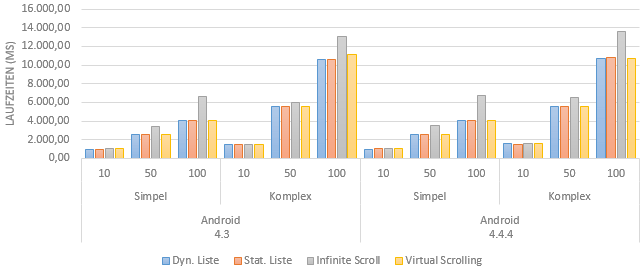
\includegraphics[scale=0.7]{Bilder/Diagramme/List-Scrollen.png}
	\caption{Listen - Laufzeitmessung Scrollen}
	\label{lists-runtime-scroll}
\end{figure}

\subsubsection{Kriterium - Two-Way Databinding}
	Das letzte untersuche Kriterium befasst sich mit der Performance während der Verwendung einer Seite durch den Anwender. Wie in Abschnitt \ref{dv-analyse} betrachtet, existiert ein enormes Optimierungspotential durch die Vermeidung von überflüssigen Two-Way-Databindings. Durch die Eigenschaften der verschiedenen Listenarten ergibt sich zum Teil automatisch eine solche Optimierung. Im Ergebnis, in Abbildung \ref{lists-runtime-digest}, ist deutlich ersichtlich, dass sowohl \gls{is} als auch \gls{vs} die Laufzeit eines \emph{\$digest}-Zyklus merklich beeinflusst. Im Vergleich zwischen statischen Listen und der \gls{vs} Technik konnte sogar eine Verbesserung von bis zu 1268\% erreicht werden. Die Ursache für solch eine enorme Steigerung ist, wie bereits erwähnt die feste Anzahl von Elementen, die sich beim \gls{vs} zur selben Zeit in der Liste befinden. Die Performance des \emph{\$digest}-Zyklus bleibt demnach nahezu konstant. Auf \gls{is} trifft diese Eigenschaft nur bedingt zu. Die Ergebnisse zeigen Laufzeiten, ohne dass die Liste zuvor durchlaufen wurde. Beim Scrollen einer Liste mit \gls{is} werden weitere Elemente fortlaufend unten angefügt. Im schlechtesten Fall verhält sich \gls{is} demnach genauso wie eine dynamische Liste. Die beste Optimierung kann für dieses Kriterium durch den Einsatz der \gls{vs} Technik erreicht werden. Im Vergleich zwischen Android 4.3 und Android 4.4.4 zeigt sich, dass Letzteres bei der Laufzeit des \emph{\$digest}-Zyklus eine bessere Performance aufweist. 
\begin{figure}[h]
	\centering
	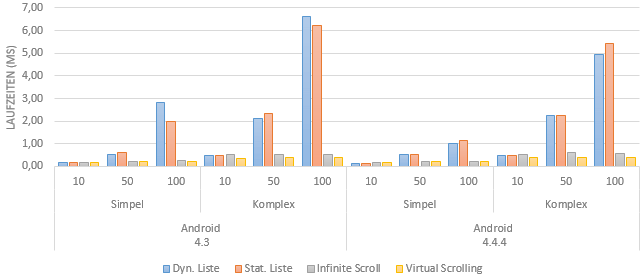
\includegraphics[scale=0.7]{Bilder/Diagramme/List-digest.png}
	\caption{Listen - Laufzeitmessung Two-Way-Databinding}
	\label{lists-runtime-digest}
\end{figure}

\subsubsection{Ergebnis}
Die einzelnen Untersuchungen haben gezeigt, dass die \gls{vs} Technik hinsichtlich aller Kriterien die beste Performance aufweist. Lediglich bei wenigen Listenelementen verhalten sich alle vier Alternativen gleich. Aufgrund der Komplexität sollten dynamische Listen bei wenigen Elementen bevorzugt werden. Sobald die Liste eine Größe von 10 - 50 Elementen überschreitet, ist die \gls{vs} Technik überlegen. Die Vorteile der \gls{is} Technik kommen insbesondere dann zum Tragen, wenn die Listenelemente nicht von Anfang an zur Verfügung stehen. Die einzige Schwachstelle, das Scrollen, kommt dabei nicht zum Tragen. Neue Listenelemente müssen ohnehin nachgeladen werden. 
\\\\
Aufgrund des Fokus dieser Arbeit bezieht sich die Argumentation auf die reine Betrachtung der Performance. Natürlich kann aufgrund von unterschiedlichen Einsatzszenarien eine bestimmte Listenart trotz Performance-Nachteilen bevorzugt werden. Beispiele dafür sind Apps wie Twitter oder Facebook. Der Nachrichtenstrom in solchen Apps hat prinzipiell kein Ende, weshalb die gängige Methodik das Nachladen neuer Elemente über eine \gls{is} Technik beinhaltet.